\section{Statement of the problem}

\subsection{Work plan}

The goal of the project is to study modern methods and develop a new version of the AlgoView system. Research is required to implement the computing component of the system. It is also required to conduct research on modern 3D visualization methods and develop an automated system for visualizing algorithm graphs. To achieve these goals, it is necessary to go through a multi-stage research and development process and complete the following tasks:

\begin{enumerate}
    \item Study the concept of an information graph of an algorithm, its properties and methods of application and analysis, study ways of describing the algorithm graph. Consider the syntax of the Algolang language, designed to describe the information structure of the algorithm in the form of an XML file. If possible, make the Algolang language more universal.
    \item Study possible processing methods and software libraries for working with information structures of the XML format, as well as methods for calculating mathematical expressions specified in text form, used in describing information graphs of algorithms.
    \item Develop software methods for processing the necessary information about the algorithm from the description in the Algolang language.
    \item Develop a new format for storing data about the algorithm, on the basis of which the information graph can be visualized without additional calculations in order to obtain the necessary information about the structure of the graph.
    \item Implement a software algorithm that, based on information obtained from the description of the algorithm in the Algolang language, composes a description of the multidimensional graph model in a new format, according to which it can be visualized. The model should be a description of the location of the vertices and edges of the graph in space, as well as the characteristics of the information graph and the properties of each element of this graph.
    \item Form the architecture of the application and the concepts of the internal representation of the algorithm graph in the AlgoView visualization system.
    \item Creation of a software tool that converts an intermediate representation of the algorithm graph in JSON format into a variety of 3D models.
    \item Implementation of software that produces interactive 3D visualization of a set of generated objects representing an algorithm graph.
    \item Creation of a web page on which visualization and interaction with the interface is carried out.
\end{enumerate}

\subsection{Intermediate data format}

The Algoview system is divided into a computational part and a visualization task. To automate the operation of the system, it is necessary to develop a new format for storing data about the algorithm. The standardized representation of the algorithm graph is a JSON structure containing the characteristics of the algorithm information graph, information about the coordinates and type of vertices, and information about the connectivity of these vertices through their unique identifiers. The developed data structure has the following form (an example of three vertices and 2 edges):

\begin{figure}
% \vspace{-0.5cm}
\centering
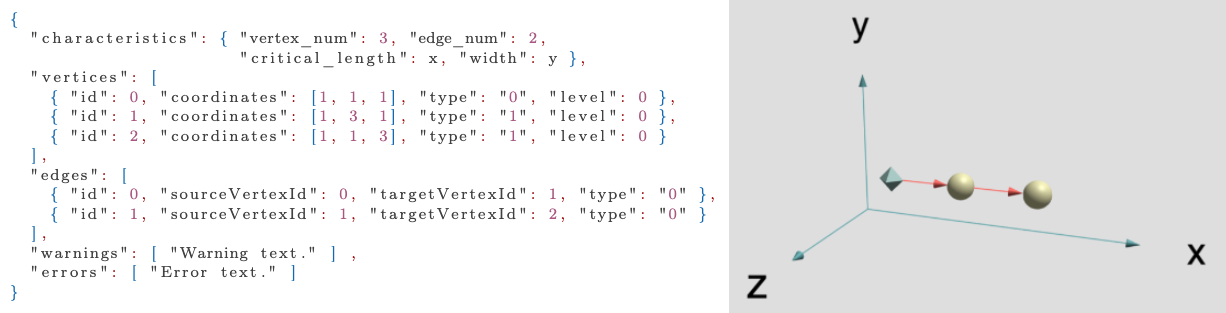
\includegraphics[height=3.1cm]{assets/json_example.png}
\caption{JSON structure, an example of the original data format and an example of visualization of this graph.}
\end{figure}

\subsection{Standard for visualizing algorithm graphs}

The Algorithm Graph Visualization Standard is a standard first described as a guide consisting of a set of rules according to which it is recommended to display an algorithm graph. The existence of the standard is determined by the need to construct images of algorithm graphs in a generally accepted form, which will be understandable regardless of the tools used to depict the graph \cite{m5}. With the advent of the AlgoView system as a universal way to generate images of algorithm graphs, many provisions in the standard require revision. Innovations in the standard concern automation of the process and relaxation of the strict requirements for the image of graphs.